% !TeX spellcheck = pl_PL
% --- W tej części należy umieścić przykład działania programu (zrzut ekranu).
\newpage
\part{\huge \textbf{Przykład działania}}
	\section*{Ekran powitalny}
		Pojawia się zaraz po uruchomieniu aplikacji. Użytkownik może uruchomić grę, wejść do jednego z\\podmenu lub wyjść z programu. W lewym górnych rogu widać aktualną liczbę klatek na sekundę.
		\begin{center}
			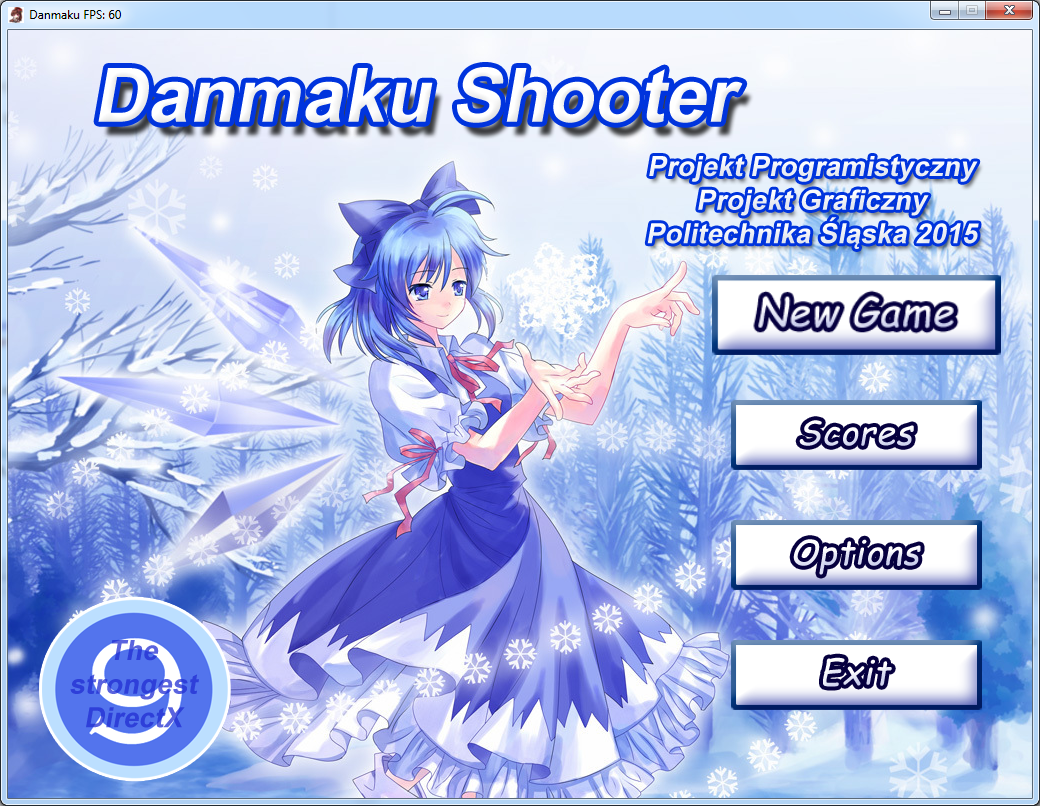
\includegraphics[width=0.7\textwidth]{./images/titlescreen}
		\end{center}
	\section*{Ekran gry}
		W czasie \textit{gameplay'u}. Porównując go z rozdziałem Treść Zadania widać, że interfejs gry jest zgodny z założeniami.
		\begin{center}
			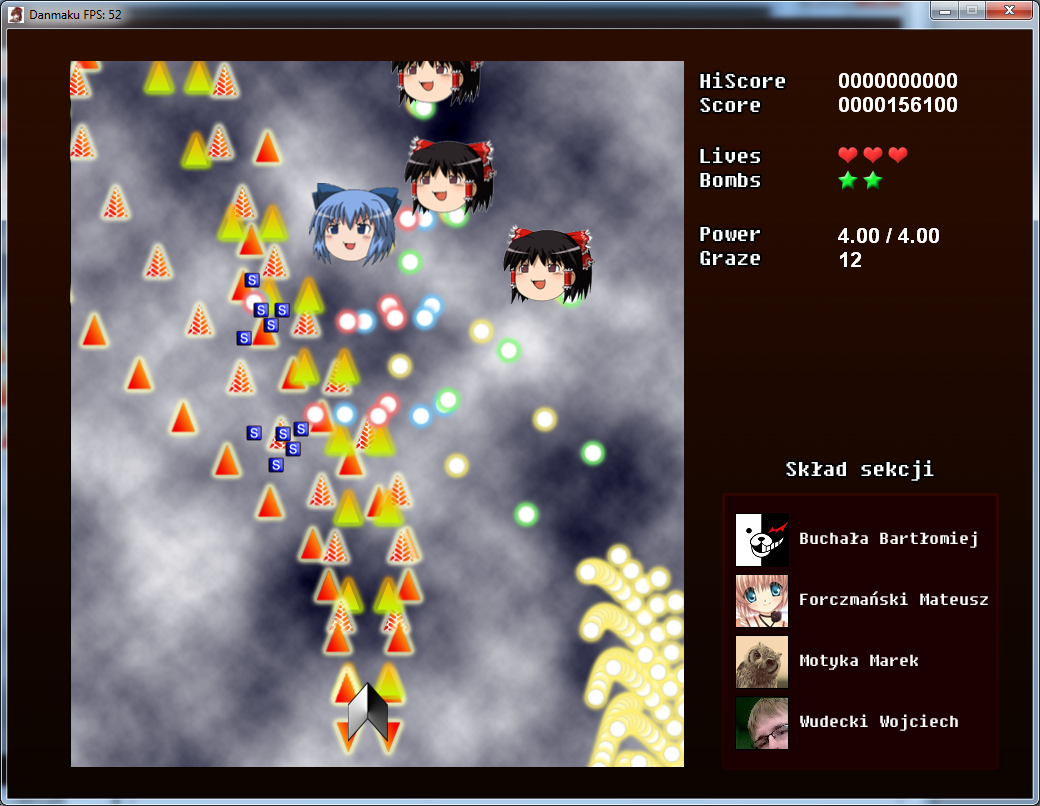
\includegraphics[width=0.7\textwidth]{./images/gameplay}
		\end{center}
		